\documentclass[12pt,a4paper,oneside,pdftex]{report}
\usepackage[utf8]{inputenc}
\usepackage[OT1]{fontenc}
\usepackage[finnish,english]{babel}

% Natbib allows you to select the format of the bibliography references.
% The first example uses numbered citations: 
\usepackage[square,sort&compress,numbers]{natbib}
% The second example uses author-year citations.
% If you use author-year citations, change the bibliography style (below); 
% acm style does not work with author-year citations.
% Also, you should use \citet (cite in text) when you wish to refer
% to the author directly (\citet{blaablaa} said blaa blaa), and 
% \citep when you wish to refer similarly than with numbered citations
% (It has been said that blaa blaa~\citep{blaablaa}).
% \usepackage[square]{natbib}

% The alltt package provides an all-teletype environment that acts
% like verbatim but you can use LaTeX commands in it. Uncomment if 
% you want to use this environment. 
% \usepackage{alltt}

% The eurosym package provides a euro symbol. Use with \euro{}
\usepackage{eurosym} 

% Verbatim provides a standard teletype environment that renders
% the text exactly as written in the tex file. Useful for code
% snippets (although you can also use the listings package to get
% automatic code formatting). 
\usepackage{verbatim}

% The listing package provides automatic code formatting utilities
% so that you can copy-paste code examples and have them rendered
% nicely. See the package documentation for details.
% \usepackage{listings}

% The fancuvrb package provides fancier verbatim environments 
% (you can, for example, put borders around the verbatim text area
% and so on). See package for details.
% \usepackage{fancyvrb}

% Supertabular provides a tabular environment that can span multiple 
% pages. 
%\usepackage{supertabular}
% Longtable provides a tabular environment that can span multiple 
% pages. This is used in the example acronyms file. 
\usepackage{longtable}

% The fancyhdr package allows you to set your the page headers 
% manually, and allows you to add separator lines and so on. 
% Check the package documentation. 
% \usepackage{fancyhdr}

% Subfigure package allows you to use subfigures (i.e. many subfigures
% within one figure environment). These can have different labels and
% they are numbered automatically. Check the package documentation. 
\usepackage{subfigure}

% The titlesec package can be used to alter the look of the titles 
% of sections, chapters, and so on. This example uses the ``medium'' 
% package option which sets the titles to a medium size, making them
% a bit smaller than what is the default. You can fine-tune the 
% title fonts and sizes by using the package options. See the package
% documentation.
\usepackage[medium]{titlesec}

% The TikZ package allows you to create professional technical figures.
% The learning curve is quite steep, but it is definitely worth it if 
% you wish to have really good-looking technical figures. 
\usepackage{tikz}
% You also need to specify which TikZ libraries you use
\usetikzlibrary{positioning}
\usetikzlibrary{calc}
\usetikzlibrary{arrows}
\usetikzlibrary{decorations.pathmorphing,decorations.markings}
\usetikzlibrary{shapes}
\usetikzlibrary{patterns}


% The aalto-thesis package provides typesetting instructions for the
% standard master's thesis parts (abstracts, front page, and so on)
% Load this package second-to-last, just before the hyperref package.
% Options that you can use: 
%   mydraft - renders the thesis in draft mode. 
%             Do not use for the final version. 
%   doublenumbering - [optional] number the first pages of the thesis
%                     with roman numerals (i, ii, iii, ...); and start
%                     arabic numbering (1, 2, 3, ...) only on the 
%                     first page of the first chapter
\usepackage[mydraft]{aalto-thesis}
%\usepackage[mydraft,doublenumbering]{aalto-thesis}
%\usepackage{aalto-thesis}



% Hyperref
% ------------------------------------------------------------------
% Hyperref creates links from URLs, for references, and creates a
% TOC in the PDF file.
% This package must be the last one you include, because it has
% compatibility issues with many other packages and it fixes
% those issues when it is loaded.   
%\RequirePackage[pdftex]{hyperref}
\RequirePackage[pdfa]{hyperref}
% Setup hyperref so that links are clickable but do not look 
% different
\hypersetup{colorlinks=false,raiselinks=false,breaklinks=true}
\hypersetup{pdfborder={0 0 0}}
\hypersetup{bookmarksnumbered=true}
% The following line suggests the PDF reader that it should show the 
% first level of bookmarks opened in the hierarchical bookmark view. 
\hypersetup{bookmarksopen=true,bookmarksopenlevel=1}
% Hyperref can also set up the PDF metadata fields. These are
% set a bit later on, after the thesis setup.   


% Thesis setup
% ==================================================================
% If you do not find the command for a text that is shown in the cover page or
% in the abstract texts, check the aalto-thesis.sty file and locate the text
% from there. 
% All the texts are configured in language-specific blocks (lots of commands
% that look like this: \renewcommand{\ATCITY}{Espoo}.
% You can just fix the texts there. Just remember to check all the language
% variants you use (they are all there in the same place). 
% ------------------------------------------------------------------
\newcommand{\TITLE}{Secure Container Runtimes for Radio Applications and Far Edge Cloud}
\newcommand{\DATE}{November 20, 2020}

\newcommand{\FTITLE}{Tietoturvallinen ohjelmistokonttien ajo radiosovelluksissa and kaukaisessa reunapilvessä}
\newcommand{\FDATE}{Marraskuu 20, 2020}

% Supervisors and instructors
% ------------------------------------------------------------------
% Usually thesis have one supervisor and one advisor. Sometimes you
% may have two advisors and, in double degree
% programs, you may have two supervisors. 
% If you have two supervisors, write both names here, separate them with a 
% double-backslash (see below for an example)
% Also remember to add the package option ``twosupervisors'' or
% ``twoinstructors'' to the aalto-thesis package (aalto-thesis.sty
% file line 72), so that the titles are in plural.

% Example of one supervisor:
\newcommand{\SUPERVISOR}{Professor Jukka Manner}
\newcommand{\FSUPERVISOR}{Professori Jukka Manner}

% If you have only one instructor, just write one name here
\newcommand{\INSTRUCTOR}{Jan Zizka M.Sc. (Tech.)}
\newcommand{\FINSTRUCTOR}{Diplomi-insinööri Jan Zizka}

% Other stuff
% ------------------------------------------------------------------
\newcommand{\PROFESSORSHIP}{Security and Cloud Computing}
\newcommand{\FPROFESSORSHIP}{Tietoturva ja pilvilaskenta}
% Professorship code is the same in all languages
\newcommand{\PROFCODE}{SCI3084}
\newcommand{\KEYWORDS}{Kata Containers, Far Edge Cloud, Mobile Edge Computing, Container, Security}
\newcommand{\FKEYWORDS}{}
\newcommand{\LANGUAGE}{English}
\newcommand{\FLANGUAGE}{Englanti}

% Author is the same for all languages
\newcommand{\AUTHOR}{Markku Leppälä}

% Currently the English versions are used for the PDF file metadata
% Set the PDF title
\hypersetup{pdftitle={\TITLE}}
% Set the PDF author
\hypersetup{pdfauthor={\AUTHOR}}
% Set the PDF keywords
\hypersetup{pdfkeywords={\KEYWORDS}}
% Set the PDF subject
\hypersetup{pdfsubject={Master's Thesis}}


% Layout settings
% ------------------------------------------------------------------

% When you write in English, you should use the standard LaTeX 
% paragraph formatting: paragraphs are indented, and there is no 
% space between paragraphs.
% When writing in Finnish, we often use no indentation in the
% beginning of the paragraph, and there is some space between the 
% paragraphs.

% Use this to control how much space there is between each line of text.
% 1 is normal (no extra space), 1.3 is about one-half more space, and
% 1.6 is about double line spacing.  
% \linespread{1} % This is the default
% \linespread{1.3}

% Bibliography style
% acm style gives you a basic reference style. It works only with numbered
% references.
\bibliographystyle{acm}
% Plainnat is a plain style that works with both numbered and name citations.
% \bibliographystyle{plainnat}


% Extra hyphenation settings
% ------------------------------------------------------------------
% You can list here all the files that are not hyphenated correctly.
% You can provide many \hyphenation commands and/or separate each word
% with a space inside a single command. Put hyphens in the places where
% a word can be hyphenated.
% Note that (by default) LaTeX will not hyphenate words that already
% have a hyphen in them (for example, if you write ``structure-modification 
% operation'', the word structure-modification will never be hyphenated).
% You need a special package to hyphenate those words.
\hyphenation{di-gi-taa-li-sta yksi-suun-tai-sta}



% The preamble ends here, and the document begins. 
% Place all formatting commands and such before this line.
% ------------------------------------------------------------------
\begin{document}
% This command adds a PDF bookmark to the cover page. You may leave
% it out if you don't like it...
\pdfbookmark[0]{Cover page}{bookmark.0.cover}
% This command is defined in aalto-thesis.sty. It controls the page 
% numbering based on whether the double-numbering option is specified
\startcoverpage

% Cover page
% These control in which language the cover-page information is shown
\coverpage{english}


% Abstracts
% ------------------------------------------------------------------
% Include an abstract in the language that the thesis is written in,
% and if your native language is Finnish or Swedish, one in that language.

% Abstract in English
% ------------------------------------------------------------------
\thesisabstract{english}{
Containerized applications have recently gained wide popularity due to portability and flexible resource allocation. However, the container runtimes provide limited isolation of workloads since the containers share the Linux kernel. Telco and radio applications handle sensitive data and need a high level of isolation and extraordinary security measures to avoid potential exploits of container runtime or kernel vulnerabilities.

Apart from the security requirements, the challenge for virtualizing radio applications is the specific requirements for container runtime features. These features include, for example, the use of accelerators, direct access to NICs, and support for multiple interfaces, which might require elevated access rights. Operating containers with elevated privileges are considered risky, as the application might escape the container.

This thesis explores Kata Containers as a potential solution for securing telco environment, as it provides runtime utilizing lightweight virtual machines running on top of a hypervisor. The solution is studied by developing an environment resembling a radio application and evaluating the I/O performance.

In this thesis, it was found out that Kata Containers provides security to telco environment supporting basic features required by the applications. Kata Containers adds overhead to the application performance while using disk-based storage volumes, which can be mitigated with design of the applications and deployment environment.
}

% Abstract in Finnish
% ------------------------------------------------------------------
\thesisabstract{finnish}{
Ohjelmistokontit sovellusten käyttöönotossa ovat saaneet paljon omaksumista viime vuosina niiden tarjoaman joustavuuden ja resurssitehokkuuden vuoksi. Ohjelmistokontit tarjoavat kuitenkin rajatun eristyksen työkuormalle sillä nämä jakavat saman Linux käyttöjärjestelmäytimen keskenään. Telekommunikaatio- ja radiosovellukset käsittelevät yksityistä dataa ja tarvitsevat vahvan eristyksen sekä kattavat turvallisuustoimet suojatakseen mahdollisilta haavoittuvuuksilta ohjelmistokonttien ajossa tai Linuxin käyttöjärjestelmäytimessä.

Tietoturvavaatimusten lisäksi haasteena virtuaalisoiduissa radio-ohjelmissa on tarkat vaatimukset ympäristön ominaisuuksissa, kuten laitteistopohjainen kiihdytys, suora yhteys verkkokorttiin ja tuki usealle samanaikaiselle käyttöliittymälle. Nämä vaatimukset saattavat vaatia korotettu käyttöjärjestelmäoikeudet, jota yleensä pidetään riskialttiina mahdollistaen käyttäjän karkaamisen ohjelmistokontista.

Tämä diplomityö arvioi Kata Containers -ohjelmistoa mahdollisena ratkaisuna tietoliikenneverkon suojaamiseen, eristäien ohjelmistokontin kevyen virtuaalikoneen sisälle. Virtuaalikonetta ajetaan virtuaalikonemonitorin päällä. Tätä ratkaisua tutkitaan radiosovelluksille tyypillisessä ympäristössä arvioiden samalla sen tukemia ominaisuuksia ja suorituskykyä.

Tämän diplomityön tuloksena on, että Kata Containers tarjoaa kattavan tietoturvallisen eristyksen tyydyttäen tietoliikennesovellusten ominaisuusvaatimukset. Suojauksen haittapuolena on suorituskyvyn heikentyminen levytallennuksessa, jota kuitenkin voidaan lieventää sovellusten ja ympäristön suunnittelulla.
}


% Acknowledgements
% ------------------------------------------------------------------
% Select the language you use in your acknowledgements
\selectlanguage{english}

% Uncomment this line if you wish acknowledgements to appear in the 
% table of contents
%\addcontentsline{toc}{chapter}{Acknowledgements}

% The star means that the chapter isn't numbered and does not 
% show up in the TOC
\chapter*{Acknowledgements}

Thanks mom!
\vskip 10mm

\noindent Helsinki, \DATE
\vskip 5mm
\noindent\AUTHOR

% Acronyms
% ------------------------------------------------------------------
% Use \cleardoublepage so that IF two-sided printing is used 
% (which is not often for masters theses), then the pages will still
% start correctly on the right-hand side.
\cleardoublepage
% Example acronyms are placed in a separate file, acronyms.tex
\addcontentsline{toc}{chapter}{Abbreviations and Acronyms}
\chapter*{Abbreviations and Acronyms}

\noindent
\begin{longtable}{@{}p{0.25\textwidth}p{0.7\textwidth}@{}}
5G & Fifth Generation \\
AR & Augmented Reality \\
AWS & Amazon Web Services \\
%CNCF & Cloud Native Computing Foundation \\
CNI & Container Network Interface \\
CRI & Container Runtime Interface \\
FEC & Far Edge Cloud \\
IoT & Internet of Things \\
%KC & Kata Containers \\
KVM & Kernel-based Virtual Machine \\
MEC & Multi-access Edge Computing \\
NIC & Network Interface Controller \\
OCI & Open Container Initiative \\
OS & Operating System \\
PV & Persistent Volume \\
RAN & Radio Access Network \\
RTT & Round Trip Time \\
SR-IOV & Single Root I/O Virtualization \\
Telco & Telecommunications \\
TLB & Translation Lookaside Buffer \\
VF & Virtual Function \\
VM & Virtual Machine \\
VMM & Virtual Machine Monitor \\
VR & Virtual Reality\\
\end{longtable}


% Table of contents
% ------------------------------------------------------------------
\cleardoublepage
% This command adds a PDF bookmark that links to the contents.
% You can use \addcontentsline{} as well, but that also adds contents
% entry to the table of contents, which is kind of redundant.
% The text ``Contents'' is shown in the PDF bookmark. 
\pdfbookmark[0]{Contents}{bookmark.0.contents}
\tableofcontents

% List of tables
% ------------------------------------------------------------------
% You only need a list of tables for your thesis if you have very 
% many tables. If you do, uncomment the following two lines.
% \cleardoublepage
% \listoftables

% Table of figures
% ------------------------------------------------------------------
% You only need a list of figures for your thesis if you have very 
% many figures. If you do, uncomment the following two lines.
% \cleardoublepage
% \listoffigures

% The following label is used for counting the prelude pages
\label{pages-prelude}
\cleardoublepage

%%%%%%%%%%%%%%%%% The main content starts here %%%%%%%%%%%%%%%%%%%%%
% ------------------------------------------------------------------
% This command is defined in aalto-thesis.sty. It controls the page 
% numbering based on whether the double-numbering option is specified
\startfirstchapter

% Add headings to pages (the chapter title is shown)
\pagestyle{headings}

% The contents of the thesis are separated to their own files.
% Edit the content in these files, rename them as necessary.
% ------------------------------------------------------------------
\chapter{Introduction}
\label{chapter:intro}

%- Tell more about the Far Edge Clouds \\
%- How the applications are run in the cloud \\
%-- Containers in the same environment not from the same origin \\
%- What features are important? \\
%-- Performance, multus, acceleration, root privileges \\


During the past years, technology companies have widely adopted virtualization technologies such as Docker. The virtualization brings a wide range of improvements to running the application on bare metal. For example, wrapped Docker container applications are highly mobile standalone applications easily deployed on any environment supporting containers with minimal overhead. Also, the virtualized application supports orchestration features such as replication and automatic deployment.

Multi-access edge computing (MEC) greatly benefits from the adaption of virtualization technologies. MEC is a crucial technology enabler for 5G technologies to serve users with low-latency and high-throughput mobile network connections. This shift enables Mobile Network Operators (MNOs) to host various applications in physical proximity to the end-users. Far Edge Cloud (FEC) takes edge computing further by closing the physical distance between to be at a maximum of 5 kilometers. The benefits to MNOs include additional revenues and higher Quality-of-experience; meanwhile, end-users enjoy low-latency, on-premise data computing, and additional location services. However, recently, it has been discovered that container architecture flaws have led to malicious applications escaping the container. As all containers share the host kernel, these malicious applications can compromise the other containers running on the same system. This compromise might lead to a breach of information from the otherwise secure applications and exposes third-part applications to each other via lateral vectors.

Kata Containers (KC) \cite{KataContainers} has been introduced as a promising solution to add an extra layer of isolation to the applications to secure the MEC platforms. The extra layer is achieved by running all containers in a lightweight virtual machine (VM). This VM adds only a little overhead to the application, as demonstrated in chapter\ref{chapter:evaluation}, but creates an application-specific kernel/hypervisor to minimize the attack surface between applications.

\section{Problem statement}
\label{section:intro_problemstatement}

The main research question of this thesis is to evaluate the performance of the architecture using Kata Containers as a secure runtime in Kubernetes orchestrated environment. The performance of Kata Containers is compared against bare metal and the current default of Kubernetes, Docker runtime. This thesis investigates the performance impact of additional isolation layer to applications with KC as runtime of Far Edge Cloud setting.

FECs support end-user devices with applications, some of which require sophisticated features such as accelerators, direct access to network interface controllers (NICs), and support for multiple parallel network interfaces. The second research question is to map out the possible gaps with the supported features of KC in the FEC setting and propose solutions to overcome the possible deficiency.

%The main research question as: Comparison of Kata Containers to runC in Kubernetes orchestrated environment. What is the performance impact of additional isolation layer to applications with Kata Containers as a runtime in Far Edge Cloud setting?

%The second research question: Are there any gaps with the supported features such as accelerators and Multus?

%One option provides for example Kata Containers which provide runtime utilizing lightweight virtual machine run on top of hypervisor. Challenge for Radio applications is that they have specific requirements on the container runtime features to allow for example use of accelerators, direct access to NICs, support for multiple interfaces (Multus), support for DPDK and ODP based data plane acceleration which require huge pages, support for dedicated and share CPU resources.


\section{Scope and Methodology}
\label{section:intro_scopemethodology}

This thesis focuses on telco applications and the needs these applications have. It is essential to focus on the performance, compatibility, and possible gaps Kata Containers might add. The majority of the applications are based on Linux operating systems, limiting the performance evaluation scope to Linux operating systems. Kata Containers is considered the potential solution for the runtime, as it is currently savoring the broadest adoption and range of features. Kubernetes is chosen as the container orchestrator for the same reason.

The first part evaluates Kata Containers concerning the FEC environment via literature review. In the second part, the performance is evaluated more practically with performance tests. The performance tests are run in an environment that is close to the specifications of the FEC environment.

\section{Results}
\label{section:intro_results}

\section{Structure of the Thesis}
\label{section:intro_structure}

Chapter \ref{chapter:cloudcomputing} describes virtualization, cloud computing and FEC environment. This chapter also discusses the requirements of Edge Cloud and the security concerns of Cloud Computing. Chapter \ref{chapter:katacontainers} focuses on the secure runtimes and Kata Containers architecture. The environment and KC are combined in a more practical chapter \ref{chapter:implementation} which implements the runtime in the FEC context and discusses the requirements to the environment and applications. The performance is evaluated thoroughly in chapter \ref{chapter:evaluation} and the performance is analyzed based on the acquired results. The last chapter \ref{chapter:discussion} focuses on the gaps in provided features, discusses the possible improvement factors, and concludes the thesis.

%MEC applications requiring low latency \\
%Security issues of containers \\
%Slowness/lack of orchestration in VMs \\
%Live migration \\
%KC as a solution \\

%Side channel leaks \\


\chapter{Background}
\label{chapter:background}

Background of virtualization needs \\
Containers \\
Security concerns of containers \\
Why VMs? \\


The problem must have some background, otherwise it is not
interesting.  You can explain the background here. Probably you should
change the title to something that describes more the content of this
chapter. Background consists of information that help other masters of
the same degree program to understand the rest of the thesis. Often
the background has two parts: the first part tells the theoretical background
and the second one describes the background tied to the implementation.

Transitions mentioned in Section~\ref{section:structure} are used also
in the chapters and sections. For example, next in this chapter we
tell how to use English language, how to find and refer to sources,
and enlight different ways to include graphics in the thesis.

\section{Language and Structure}

Moreover, the transitions are also used in the paragraph and the
sentence level meaning that all the text is linked together. For example,
the word ``moreover'' here is one way, but of course you should use
variation in the text. Examples of transitional devices (words) and
their use can be found from writing guides, e.g. from the Academic
writing instructions of Aalto
University Language Center
\footnote{http://sana.aalto.fi/awe/ and especially for connecting words 
http://sana.aalto.fi/awe/cohesion/signposts/index.html/} of
Purdue University or Strunk's Elements of
Style\footnote{http://www.bartleby.com/141/}. Remember that footnotes
are additional information, and they are seldom used.  If you refer to a source, you do no
not use footnote. The right command for the references is \emph{cite},
and we will discuss about that later in this Chapter. 

Language Center of Aalto University offers many good courses for
thesis writes. For example, LC-1320 Thesis Writing for Engineers (MSc)
is planned to support writing the master's thesis 
and LC-1310 Academic Communication for MS Students covers both oral
and written language.

The language used in the thesis should be technical (or
scientifical). For example, the abreviations aren't used but all them
are written open (i.e. ``are not''). Since the content itself is often
hard to understand (and explain), the sentences should not be very
long, use complex language with several examples embedded in the same
sentence, and, also, seldom used words and weird euphemism or paraphrases
can make the sentence hard to follow and to read it with only one
time, and making everything even harder to understand all this without
any punctuation marks makes the instructor cry and finally after
trying to correct the language, you will get boomerang, and everyone's
time has just been wasted.

You can translate your latex file to rtf with the \texttt{latex2rtf} command in the
kosh.aalto.fi shell server. Then, the line breaks
will not be problems for the proofreader of Word.

Note also that if you have a section or a subsection, you have to have
at least two of them, or otherwise the section or subsection title is
unnecessary. Same with the paragraphs: you should not have sections
with only one paragraph, and single sentence paragraph.

\subsection{Finding sources}

Good starting points for finding references in computer science are: 
\begin{itemize}
% You can use this command to set the items in the list closer to each other
% (ITEM SEParation, the vertical space between the list items) 
\setlength{\itemsep}{0pt}
\item Aalto library's Computer Science Guide: \url{http://libguides.aalto.fi/computer} 
(in English) and \url{http://libguides.aalto.fi/tietotekniikka} (in Finnish)
\item Finna Portal (Aalto Library): \url{https://aalto.finna.fi/?lng=en-gb} (in English) 
and \url{https://aalto.finna.fi/} (in Finnish)
\item ACM Digital library: \url{http://portal.acm.org/}
\item IEEExplore: \url{http://ieeexplore.ieee.org}
\item ScienceDirect: \url{http://www.sciencedirect.com/}
\item \ldots although Google Scholar (\url{http://scholar.google.com/}) will
find links to most of the articles from the abovementioned sources, if you
search from within the university network
\end{itemize}

Sometimes the Finna Portal can also help getting the whole article instead of just the abstract.
The library has also a self-study guide to information retrieval~\cite{howfindinfo}.

\subsection{Sources and reference list}

Aalto library has a comprehensive citation guide
~\cite{bibinstructions}.

The other bibliographic styles are also used in the CS field. For example, usability
uses the Harvard style where instead of numbers, the reference is
marked into the text with author's name and publishing year. You can
change the bibliography style in the thesis-example.tex file. You get
the normal text reference, e.g. (Haapasalo, 2010), with latex command
\texttt{citet} or the plain \texttt{cite}, and with command
\texttt{citep}, you get the text reference ``Haapasalo (2010)'' that
you can use as subject of a sentence. Next, we tell more about how to mark
the references in the text.

\subsection{Referring to sources}

\emph{Haapasalo~\cite{HaapasaloThesis} researched database algorithms
  that allows use of previous versions of the content stored in the
  database.} This kind of marking means that this paragraph (or until
the next reference is given) is based on the source mentioned in the
beginning.  Giving the source you should use only the family name of
the first author of the article, and not give any hints about what is
the type of the article that is referred nor its title.

\emph{B+-trees offers one way to index data that is stored in to a
  database. Multiversion B+-trees (MVBT) offer also a way to restore
  the data from previous versions of the database. Concurrent MVBT
  allows many simultaneous updates to the database that is was not
  possible with MVBT.~\cite{HaapasaloThesis}} When the marking is
after the period, the reference is retrospective: all the paragraph
(or after previous reference marking) is based on the source given in
its end. If the content is very broad, you can start with saying
\emph{According to Haapasalo}, then continue referring the source with
several separate sentences, and in the end put the marking of your
source \emph{ that shows that CMVBT are the
  best. ~\cite{HaapasaloThesis}}. 

If your paragraph has several sources, the above mentioned styles are
not proper. The reader of your thesis cannot know which of your
sources give which of the statements. In this case, it is better to
use more finegraded refering where the reference markings that are
embedded in the sentences. For example, \emph{the multiversion B+-tree
  (MVBT) index of Becker et al.~\cite{becker:1996:mvbt} allows database
  users to query old versions of the database, but the index is not
  transactional.
  It's successor, the transactional MBVT (TMVBT), allows a single transaction
  running in its own thread or process to update the database concurrently
  with other transactions that only read the
  database~\cite{haapasalo:2009:tmvbt}. 
  Further development, titled the concurrent MBVT (CMVBT),
  allows several transactions to perform updates to the database at the same
  time~\cite{HaapasaloThesis}}. 
  Here, the references are marked before
  the period in the sentences where they are used. You should never
  but all these sources in the end of the paragraph. Referring several
  source at once should only used when you give a set of examples.

Finally, direct quotes are allowed. However, often you should avoid
them since they do not usually fit in to your text very well. Using
direct quotes has two tricks: quotation marks and the source.  \emph{
  ``Even though deletions in a multiversion index must not physically
  delete the history of the data items, queries and range scans can
  become more efficient, if the leaf pages of the index structure are
  merged to retain optimality.''~\cite{HaapasaloThesis}} Quotes are
hard to make neatly since you should use only as much as needed
without changing the text. Moreover, you often do not really
understand what the author has mentioned with his wordings if you
cannot write the same with your own words. Remember also that never
cut and paste anything without marking the quotation marks right away,
and in general, never cut and paste anything at all!

\chapter{Environment}
\label{chapter:environment}

Telecommunications computing ... The computing locates in various data centers as described in Figure \ref{fig:AirFrame}. Central data centers are built to massive warehouses that take advantage of centralized maintenance and 

Telco environment
Central data center vs far edge cloud in general

\begin{figure}[ht]
  \begin{center}
    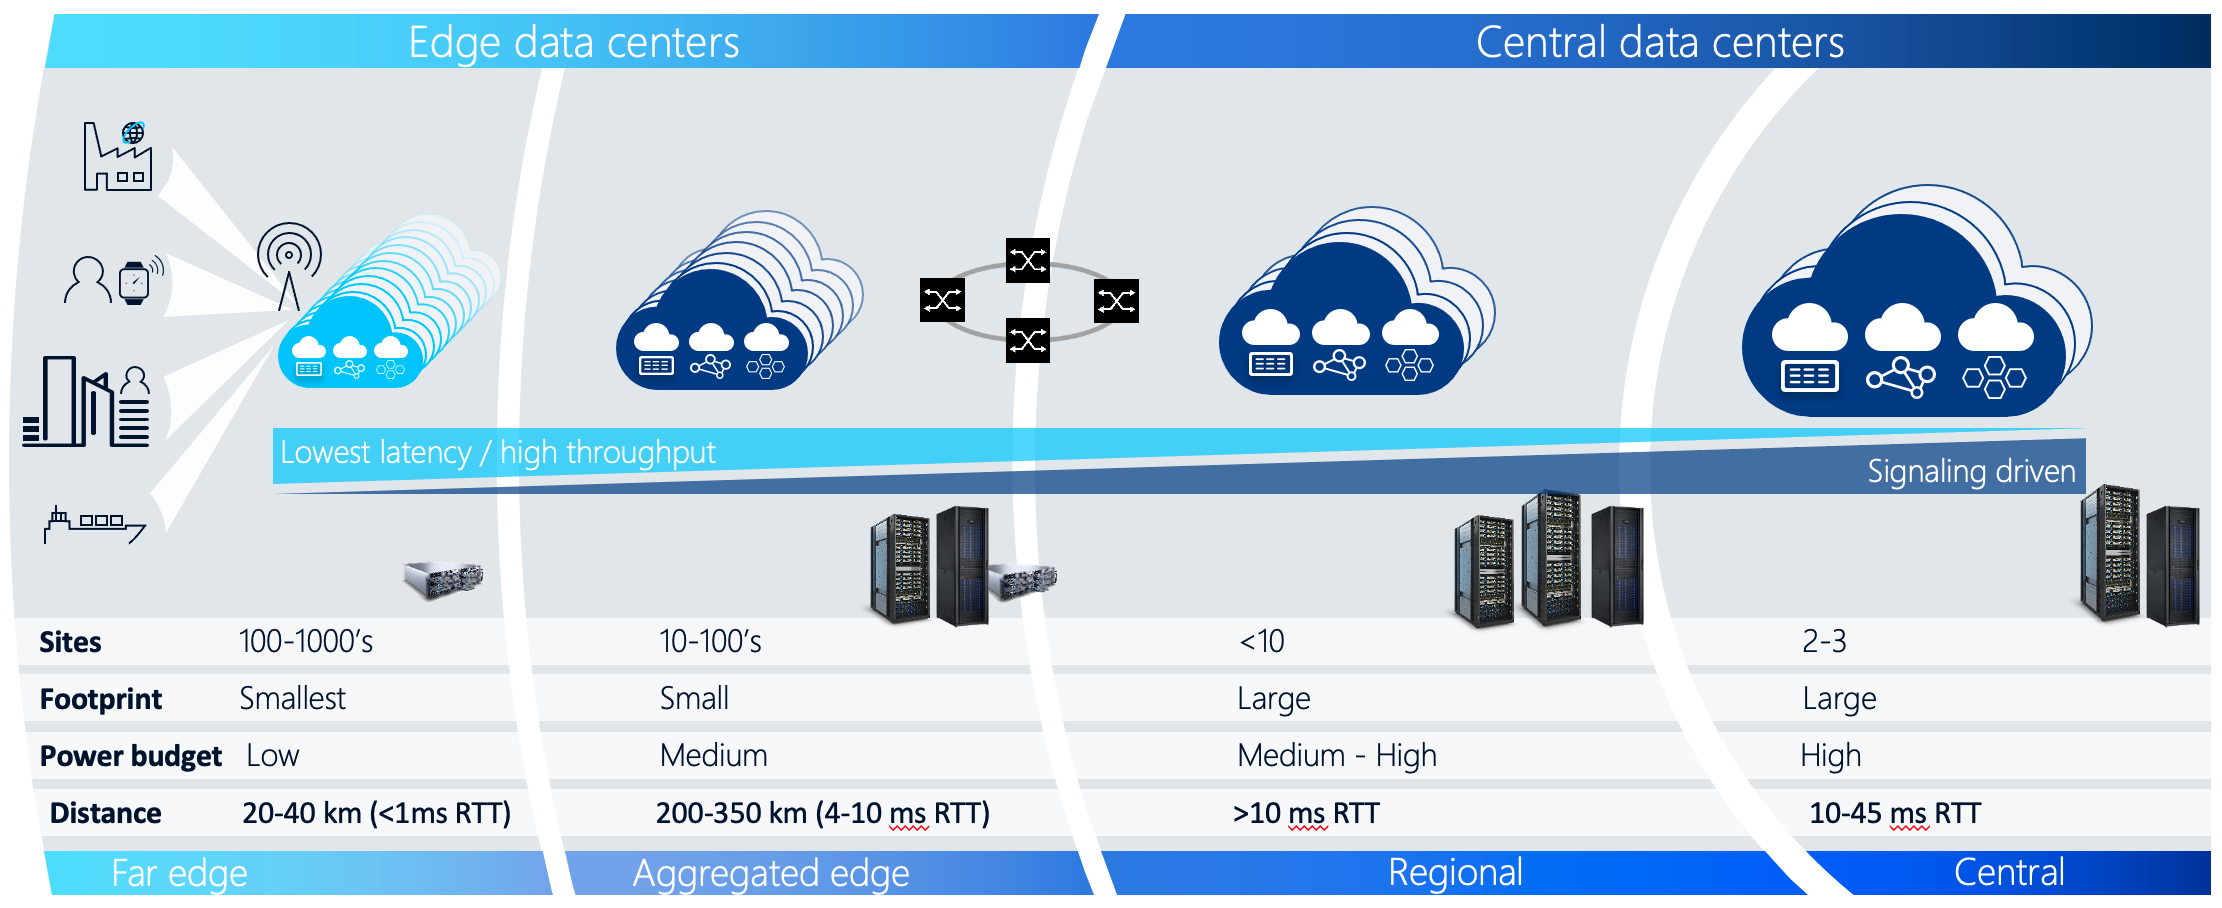
\includegraphics[width=13.5cm]{LaTeX/images/AirFrame.png}
    \caption{Far edge comparison to central data center \cite{AirFrameOpenEdgeServer}}
    \label{fig:AirFrame}
  \end{center}
\end{figure}

\section{Multi-access Edge Computing}

Multi-access Edge Computing (MEC) places compute and storage resources in the Radio Access Network (RAN) improving the delivery of content and applications to end user. MEC improves network efficiency by processing data on the mobile network cell instead of hauling it completely back to regional or central data centers for processing. The data can be processed partially or completely on the MEC node. For example, large public venues, such as stadiums or arenas, are good candidates for MEC, especially where localized venue services are important. In this use case, video created at a sports event or concert is served to on-site consumers from a MEC server, running appropriate applications located on the stadium premises. This video traffic is locally stored, processed and delivered directly to users at the event and does not require backhaul to a centralized core network and to then be returned to the user at the venue. The local processing of data reduces perceived latency on end-user and limits stress on the backhaul network. \cite{Brown2016}

Efficient capacity vs low latency & efficient transport

MEC covers two edge entities: aggregated edge and far edge. Aggregated edge locates usually at most 200 to 350 kilometers away from the end user and promises 4 to 10 millisecond round trip time (RTT).

\subsection{Far Edge Cloud}

Benefits of far edge
    - Latency
    - Allowing thin clients / offloading task to edge
    - Price and effect to environment
    - Security
    - Centralized repairing / upgrading (?)
    - Less power consumption
    - Flexibility in installment
    



\subsection{Applications}


\subsection{SR-IOV}
\label{section:SR-IOV}

I/O performance is critical to high performance telco systems. I/O intensive servers may waste CPU cycles, waiting for I/O data or spinning on idle cycles, which reduces system performance and increases latency. Single Root I/O Virtualization (SR-IOV) standard allows an I/O device, such as network interface controller (NIC), to be shared by multiple VMs. The SR-IOV technology is a hardware based virtualization solution that improves both performance and scalability. \cite{Dong2012}

Traditionally, when a guest accesses the I/O device, VMM needs to intervene in the data processing to share the physical device. The VMM intervention leads to additional I/O overhead for a guest OS. SR-IOV provides hardware enhancements for the Peripheral Component Interconnect Express (PCIe) device, which aims to remove major VMM intervention for performance data movement, such as the packet classification and address translation. An SR-IOV-capable device is able to create multiple light-weight instances of PCI function entities, known as Virtual Functions (VF). Each VF can be assigned to a VM for direct access, but still shares major device resources, achieving both resource sharing and high performance. \cite{Dong2012}





Requirements
- Root
- SR-IOV
- NICS

- Environment in MEC application
    - How migrated?
    - Elevated privileges and other requirements compared
    - Something else?
Nokia's environment \\
Usage of KC in Nokia's environment \\





% Comment: If your sentence ends in a capital letter write \@ before the period

% If you do need a normal space after a period (instead of
% the longer sentence separator), use \  (backslash and space) after the
% period. Like so: a.\ first item, b.\ second item.

\chapter{Kata Containers}
\label{chapter:katacontainers}

Securing container runtime is a crucial task in MEC in order to run multiple instances in the same edge securely. Container escapes\cite{CVE-2019-5736}\cite{CVE-2020-14386} are exposing other instances residing in the platform. Therefore, multiple solutions have been developed to provide stronger workload isolation using hardware virtualization technology as a second layer of defense. One of the most prominent approach includes wrapping the container inside a micro VM, which is a lightweight version of traditional VM with minimal overhead. The dedicated kernel of micro VM, provides isolation of network, I/O and memory and can utilize hardware-enforced isolation with virtualization extensions. In this Thesis, we will focus on Kata Containers as a secure container runtime. Kata Containers perform like containers, but provide the workload isolation and security advantages of VMs. It combines the benefits of containers and VMs. \cite{KataContainers}

Kata Containers has originated from Intel's Clear Containers \cite{ClearContainers} and Hyper runV \cite{runV} in December 2017. KC is open source and licensed under the Apache 2.0 license. The development is driven by an Architecture Committee. This committees members are elected by contributors, oversees architectural decisions, including standardization, and resolves technical disagreements between project maintainers. Currently this committee is comprised of five members from Apple, Intel, Ant Financial, and Red Hat. \cite{KataContainersGovernance} \cite{KataContainers}

\section{Architecture}

In this Thesis environment, Kata Containers is deployed within Kubernetes. Figure \ref{fig:KataContainersArchitecture} demonstrates the latest architecture defined version 2.0. The architecture is comprised of six elements: Kubernetes, containerd, Kata Shim V2, Hypervisor, Agent, and Virtual Machine.

Kata Containers is Open Container Initiative (OCI)\cite{OCI} compliant runtime, thus it obeys OCI runtime specification and supports all the OCI runtime operations. As any OCI compliant runtime, the KC works seamlessly with the Kubernetes Container Runtime Interface (CRI)\cite{CRI} through the CRI-O or containerd implementation.

\begin{figure}[ht]
  \begin{center}
    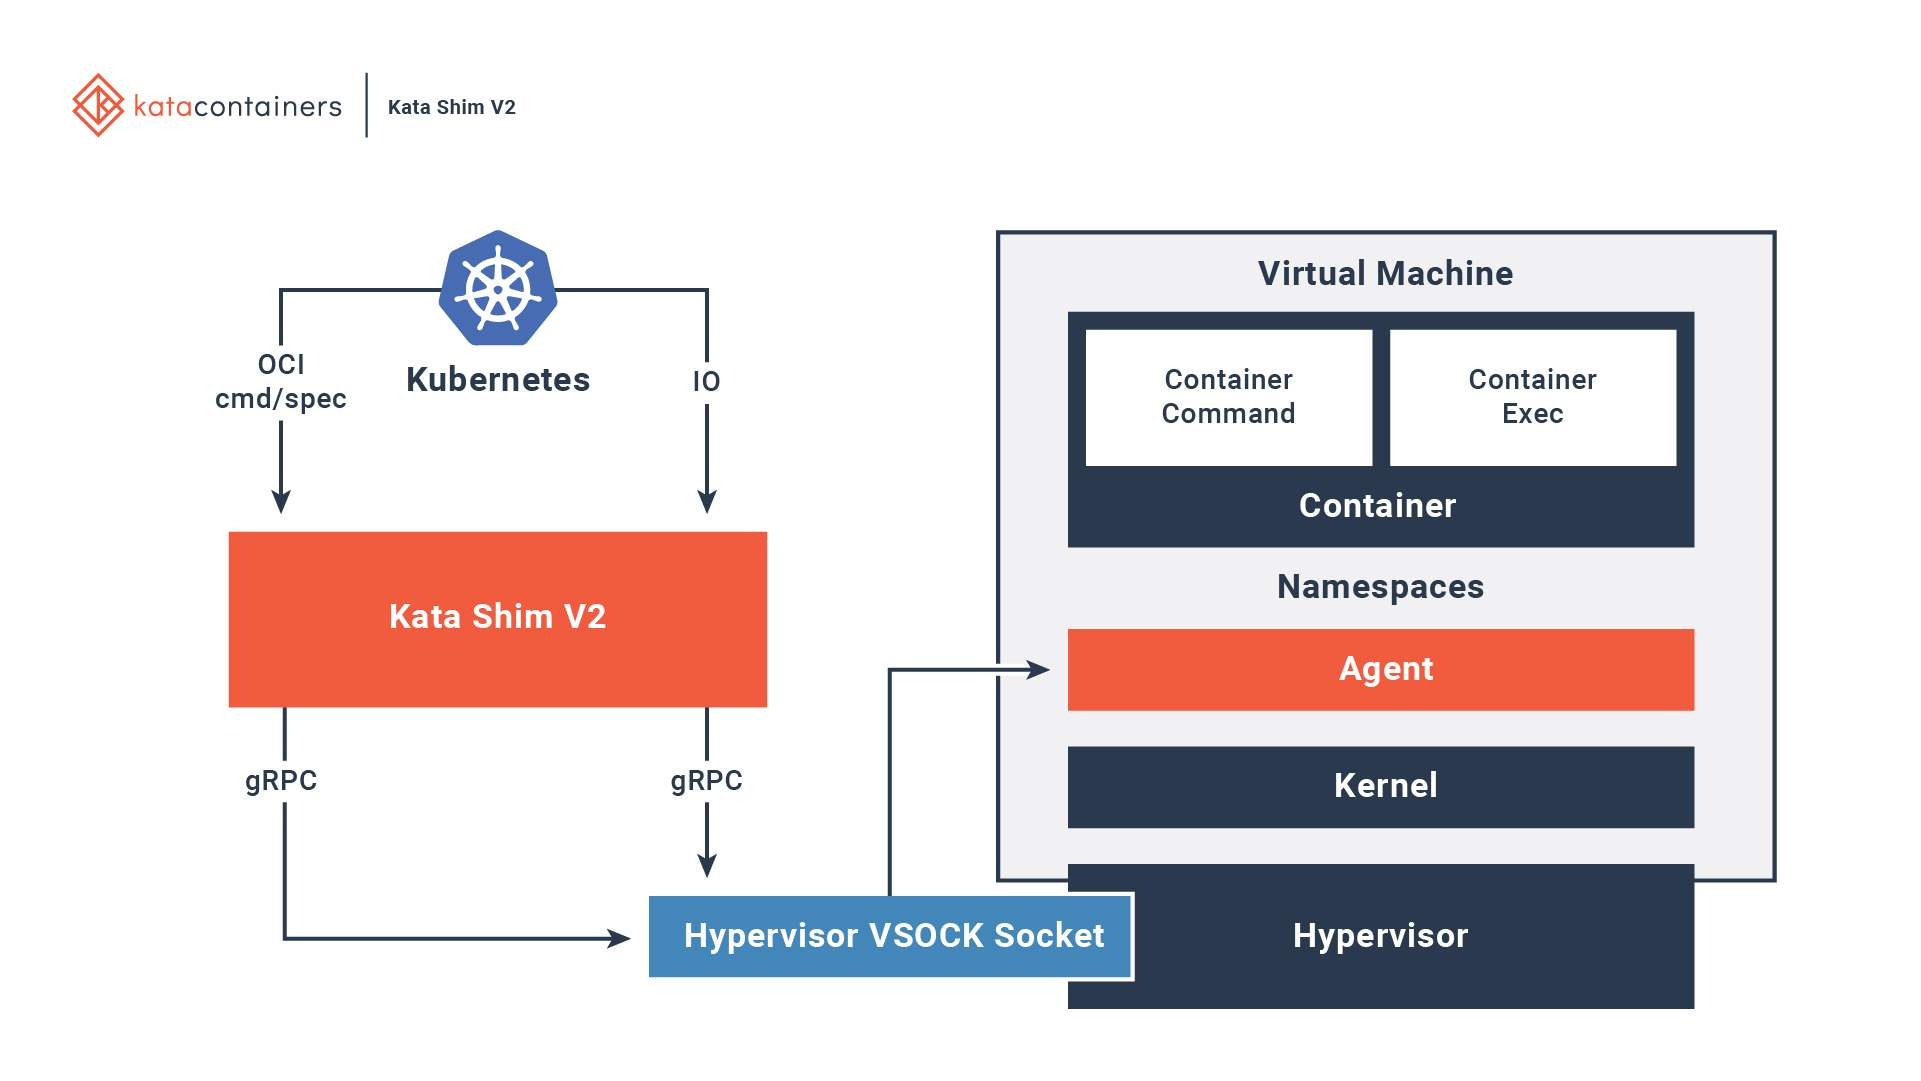
\includegraphics[width=13.5cm]{LaTeX/images/KataContainersArchitecture.jpg}
    \caption{Kata Containers 2.0 architecture \cite{KataContainers}}
    \label{fig:KataContainersArchitecture}
  \end{center}
\end{figure}

\begin{figure}[ht]
  \begin{center}
    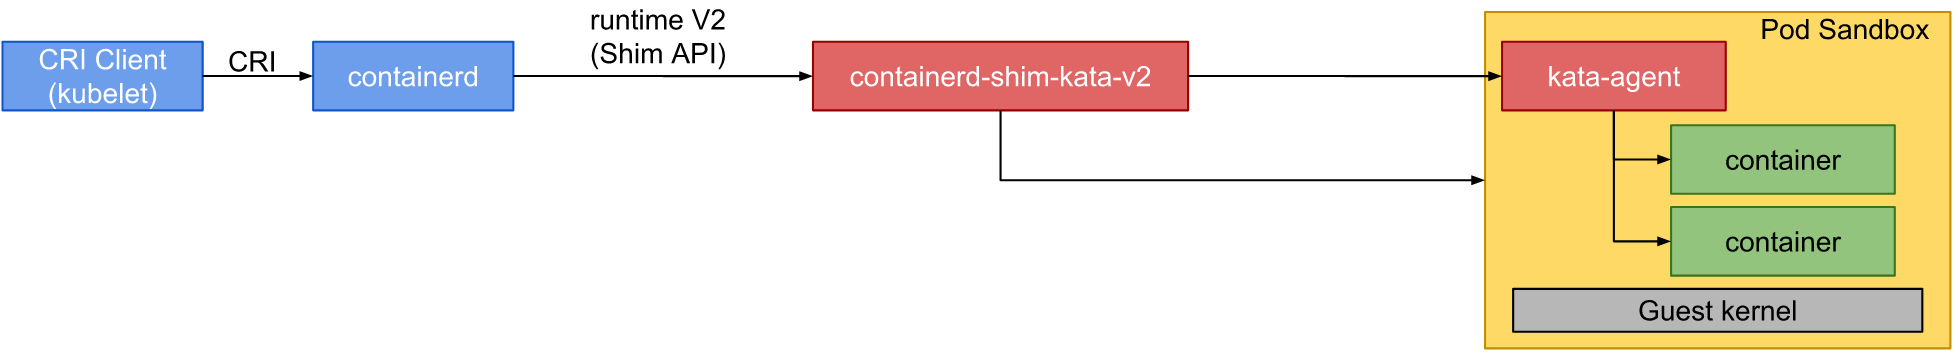
\includegraphics[width=13.5cm]{LaTeX/images/KataContainersComponents.png}
    \caption{Kata Containers 2.0 components \cite{KataContainersArchitecture}}
    \label{fig:KataContainersComponents}
  \end{center}
\end{figure}

\subsection{Kubernetes}

Kubernetes acts as an container-orchestration system for automating deployment, scaling, and management of containerized applications \cite{Kubernetes}. Kubernetes offers flexible configuration and it can installed inside a VM or on bare-metal. Like most distributed computing platforms, a Kubernetes cluster consists of at least one master node and multiple compute nodes. Each node runs a container runtime, such as Docker or containerd, along with an agent that communicates with the master.

Each container is launched as a pod. Pods are the atomic unit on the Kubernetes platform. A single node can include multiple pods inside it, and each pod is tied to the node it is created within. A runtime can be selected on a pod level, thus a single node can consists of workloads with various runtimes. This comes handy, whenever non-confidential, but highly performance-centric applications needs to be deployed in a node within more security oriented applications.

\subsection{Containerd}

Containers inside Kubernetes are managed via a container runtime. Containerd is an implementation of the Kubernetes CRI to enable using OCI compatible runtimes. It is an industry-standard container runtime with an emphasis on simplicity, robustness and portability. It is available as a daemon for Linux and Windows, which can manage the complete container lifecycle of its host system. The flexibility of containerd allows Kubernetes to register and use various OCI-compliant runtimes, such as Kata Containers, as container runtime for running pods. Containerd supports multiple means to download images including trust and image verification. Containerd also manages container process lifecycles, low-level storage, and resource isolation as required by the CRI. \cite{containerdGithub}\cite{containerd}

\subsection{Kata Shim V2}

The primary deliverable of the Kata Containers project is a CRI-friendly shim. The shim launches container runtime, which launches the container itself. The shim enables for daemonless containers, thus allowing runtime to exit after the container has been launched, and then becomes the parent of the container. \cite{Crosby}

\subsection{gRPC and ttRPC}

gRPC is a high performance Remote Procedure Call framework that can run in any environment. It connects services in and across data centers with pluggable support for load balancing, tracing, health checking and authentication. This protocol allows the runtime to send container management commands to the agent. The protocol is also used to carry the I/O streams such as stdout, stderr, and stdin, between the containers and manage the engine, which is containerd in this Thesis. \cite{gRPC}\cite{KataContainersArchitecture}

However, gRPC requires a lot of memory overhead for importing packages and at runtime. While this is great for many services with low density requirements, this can be a problem when running a large number of services on a single machine or on a machine with a small amount of memory. ttRPC also offers harnessed security by limiting attack surface and improved observability via metrics about the runtime itself, the VMM, as well as the guest kernel. Kata Shim V2 offers the support for ttRPC protocol to communicate with the agent. \cite{ttRPC}

\subsection{Hypervisor}

The VM of Kata Containers instance is launched by Virtual Machine Monitor (VMM). VMM consists of Virtual Machine Manager and a hypervisor. Kata Containers currently supports four different VMMs: ACRN hypervisor, Cloud Hypervisor, QEMU, and Firecracker. All these VMMs are open source projects.

ACRN is a reference hypervisor, which is built to meet the needs of embedded IoT development. It is developed with low overhead,fast boot-up, and configurations to support variety of devices and deployment scenarios. ACRN is a type 1 reference hypervisor stack that runs on bare-metal hardware, addressing the gap that currently exists between data center hypervisors, and hard partitioning hypervisors. \cite{ACRN}

Cloud Hypervisor is a VMM that runs on top of Kernel-based Virtual Machine (KVM). The project focuses on exclusively running modern, cloud workloads, on top of a limited set of hardware architectures and platforms. Cloud workloads refers to those that are usually run by customers inside a cloud provider, and most I/O are handled by performant para-virtualized devices, such as Virtio. \cite{CloudHypervisor}

QEMU is a generic machine, userspace emulator, and virtualizer. QEMU is capable of emulating a complete machine in software without any need for hardware virtualization support. It can also integrate with the Xen and KVM hypervisors to provide emulated hardware while allowing the hypervisor to manage the CPU. \cite{QEMUGithub}\cite{QEMU}

Firecracker VMM is developed by Amazon Web Services (AWS). Firecracker uses KVM to launch workload in lightweight micro virtual machines. Of Amazon's cloud products, Firecracker is deployed at least in AWS Lambda and Fargate. Firecracker currently supports Intel CPUs, with AMD and Arm support in developer preview. \cite{AWS}\cite{FirecrackerDesign}\cite{Debab2021}

\subsection{Agent}

Agent, also known as Kata-Agent, resides inside the Kubernetes pod in the computing node and its main task is to spawn the container process. The agent process runs as a daemon inside the virtual machine. This agent runs a ttRPC or gRPC server in the guest using a Virtio serial or VSOCK interface which the VMM exposes as a socket file on the host. \cite{KataContainersArchitecture}


\subsection{Container}

- How container content is affected by Kata. Any requirements? Performance degradation?


\section{Isolation and resource allocation}

\begin{figure}[ht]
  \begin{center}
    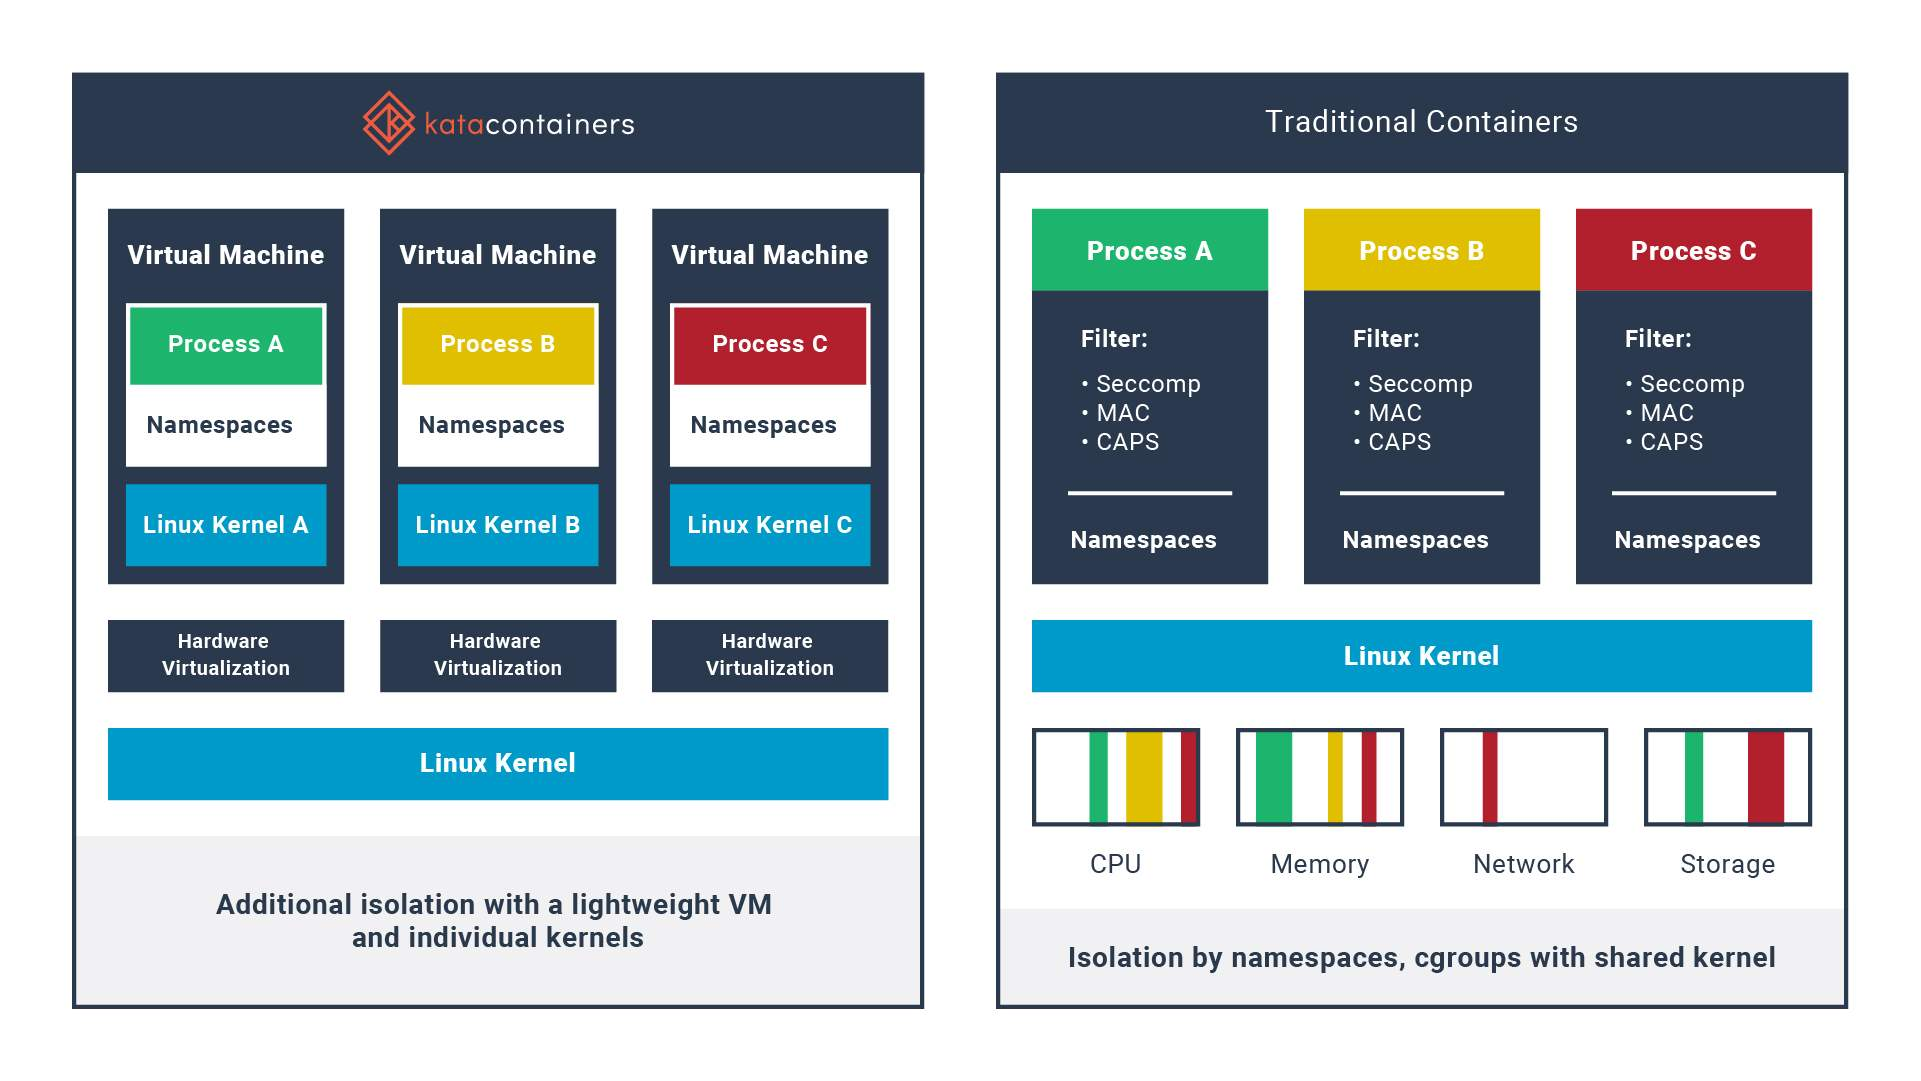
\includegraphics[width=13.5cm]{LaTeX/images/KataContainersStack.jpg}
    \caption{Kata Containers stack vs traditional container stack\cite{KataContainers}}
    \label{fig:KataContainersStack}
  \end{center}
\end{figure} 

\section{Networking}

\section{Related work}

Kata Containers is not the sole option providing secure container runtime nor isolation in the container kernel layer. Microsoft offers a container instance isolation option inside Azure with Hyper-V. The hardware isolation is based on VMs, likewise in KC and Firecracker, thus leveraging the additional kernel layer. \cite{Hyper-V}

gVisor provides a second isolation method, differing from Kata Containers and Firecracker. gVisor intercepts application system calls and acts as the guest kernel without translating through virtualized hardware. The architecture can be thought of as a merged kernel and VMM. gVisor includes OCI runtime runsc, which provides the isolation boundary between the application and host kernel. Google develops gVisor, and it is harnessed in various Google's cloud products such as Kubernetes Engine \cite{GKE} and Cloud Run \cite{CloudRun}. \cite{Debab2021}\cite{gVisor}

A third approach for container isolation is IBM Nabla\cite{Nabla}. Nabla containers use library OS, also known as unikernel, to avoid system calls and reduce the attack surface. Nabla is based on a custom VMM named Nabla Tender to manage lightweight VMs executing unikernels. Nabla containers only use seven system calls, blocking all others via a Linux \texttt{seccomp} policy. The Nabla Tender intercepts hypercalls related to storage and network from unikernel VMs and translates them into syscalls to the host. \cite{Debab2021}

All the before-mentioned projects are open source and actively maintained. However, Nabla seems to be slightly less active in comparison to the other projects. Commercial and enterprise cloud platforms, such as AWS, uses Firecracker, and GKE uses gVisor. However, it is unknown for security reasons which approaches are used in the other platforms to isolate containers.


% that it fits to the same space as the text (total width = \textwidth).
% If you do need more space, you can either
% 1) ignore the LaTeX warnings 
% 2) use the textpos-package to manually position the table (read the package
%    documentation)
% 3) if you have the table as a PDF document (of correct size, A4), you can use
%    the pdfpages package to include the page. This overrides the margin
%    settings for this page and LaTeX will not complain.
% ------------------------------------------------------------------
% Another note:
% ------------------------------------------------------------------
% If your table fits to \textwidth, but the cells are so narrow that the text
% in p{..}-formatted cells does not flow nicely (you get underfull warnings 
% because LaTeX tries to justify the text in the cells) you can manually set
% the text to unjustified by using the \raggedright command for each cell 
% that you do not want to be justified (see the example below). \raggedleft 
% is also possible, of course...
 
\chapter{Implementation}
\label{chapter:implementation}

Methodology \\
How KC was implemented in the MEC/NESC \\
How it filled the requirements? \\
- NIC, hardware acceleration, Multus? \\


\chapter{Evaluation}
\label{chapter:evaluation}

Performance evaluation \\
- Methodology \\
- How/what is tested \\
    - Hypervisors
- Results \\
- Evaluation \\
- Comparison to other providers (AWS, GCP...) \\






The extra layer of security provided by Kata Container's micro-VM comes with a price of degraded performance and computational overhead. Previous work, such as \cite{Kumar2020} and \cite{EverartsdeVelp2020} have examined the performance, when compared Kata Containers against native runtime runC, the most common OCI-compliant runtime. In these two papers, Kata Containers architecture design results in performance decrease in IO throughput, and in memory and CPU utilization. However, the results in these papers are highly dependant on the specific test environment and do not take in account the latest development of Kata Containers performance provided by the runtime version 2.0 released in December 2020. In this paper, the system performance evaluated in environment simulating a telco architecture, which is discussed in Section \ref{section:test_architecture}.

\section{Test architecture}
\label{section:test_architecture}

The test environment simulates multiple relations that are most common in a telco environment. The test environment cluster is described in Figure \ref{fig:TestArchitectureCluster} and Node 1 in more detail in Figure \ref{fig:TestArchitectureNode}. The cluster consists of two nodes, which both have two containers inside. The difference between nodes are pods, with Node 1 consisting of a single pod with two containers inside, and Node 2 consist of two pods with a single container deployed to each pod. The purpose of the heterogeneous environment is to evaluate performance of a single container or between two containers in various scenarios. SR-IOV visualized in Figure \ref{fig:TestArchitectureNode} is described in detail in Section \ref{section:SR-IOV}.

\begin{figure}[ht]
  \begin{center}
    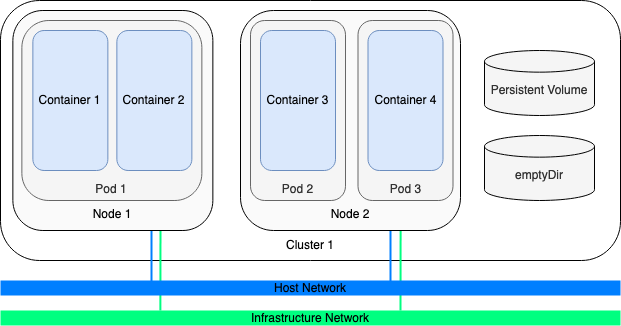
\includegraphics[width=13.5cm]{LaTeX/images/TestArchitectureCluster.png}
    \caption{Kubernetes test cluster overview}
    \label{fig:TestArchitectureCluster}
  \end{center}
\end{figure}

\begin{figure}[ht]
  \begin{center}
    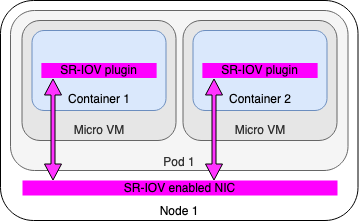
\includegraphics[width=13.5cm]{LaTeX/images/TestArchitectureNode.png}
    \caption{Node test cluster with two containers in a single pod}
    \label{fig:TestArchitectureNode}
  \end{center}
\end{figure}

\subsection{Containers}

Container - container inside pod

Container - container between pods

Container - container across nodes and a pods

Container - storage

\subsection{Storage}

The cluster consists also two storage options, which are Persistent Volume (PV) and emptyDir. PV 
    - What is emptyDir?
    - PV (block). Why block? Link to K8s docs.
    - Volumes mounted.
    - Multi-tenancy? Write many?

\subsection{Networking}

Networking
    - Two networks. What is the difference?
    - Access to storage not via network, unless NFS(?).













\section{Methodology}

The test environment is hosted by a dedicated server which is built and tailored to support edge and far-edge cloud deployments.


\section{Results}

\section{Evaluation}

\section{Benchmark from other platforms}
 
\chapter{Discussion}
\label{chapter:discussion}

How was the performance? \\
What should be improved? \\
 
\chapter{Conclusions}
\label{chapter:conclusions}


% Load the bibliographic references
% ------------------------------------------------------------------
% You can use several .bib files:
% \bibliography{thesis_sources,ietf_sources}
\bibliography{sources}

\end{document}
